\chapter{Квазиклассическое приближение}

Точное решение уравнение Шрёдингера (УШ) в квантовой механике возможно лишь для ограниченного числа задач, в то время как подавляющее большинство задач решается \underline{приближенными методами}. В качестве примера таких методов выступает \underline{квазиклассическое приближение}.

Это приближение позволяет сформулировать метод приближенного решения УШ, основанный на использовании малости постоянной Планка $\hbar$.
 
\section{Критерий применимости квазиклассического приближения}

Предварительное изучение квантовой механики показывает, что при $\hbar \to 0$ законы квантовой механики должны перейти в классические, что обеспечивается принципом соответствия, на котором мы основывались при выводе ряда положений квантовой механики (см. \textsection\textsection 2,3 гл. 5). Необходимо выяснить, как следует понимать, что классическое приближение хорошо описывает физические явления, когда величиной кванта действия $\hbar$ можно пренебречь.

\subsection{Переход к уравнению Гамильтона-Якоби}

При решении уравнение Шрёдингера
$$
i\hbar \pd{}{t} \Psi(\vr, t) = \brcr{-\frac{\hbar^2}{2m} \nabla^2 + U(\vr)} \Psi(\vr,t)
$$

используем подстановку:
$$
\Psi = \mathcal{A} e^{\frac{i}{\hbar}S(\vr,t)}
$$

Здесь $S(\vr, t)$ - пока неизвестная функция, имеющая как и $\hbar$ размерность действия. Известно, что в классической мехинике действие вещественно, тогда как в используемой подстановке функция $S(\vr, t)$, вообще говоря, может быть и комплексной. Получим уравнение, которому удовлетворяет $S(\vr, t)$:   

$$
\nabla \Psi(\vr,t) = \brc{\frac{i}{\hbar}\nabla S}\Psi
$$
Подставим $\Psi$ и $\nabla \Psi$ в уравнение Шрёдингера:
$$
i\hbar\brc{\frac{i}{\hbar}\pd{S}{t}}\Psi = 
\brcr{ -\frac{\hbar^2}{2m} \brs{ \brc{\frac{i}{\hbar}\nabla S}^2 + \frac{i}{\hbar}{\nabla^2} S} + U(\vr) } \Psi,
$$
откуда следует
\begin{equation}
\label{eq:11_1_1}
\boxed{-\pd{S}{t} = \frac{(\nabla S)^2}{2m} + U(\vr) - \frac{i\hbar}{2m} (\nabla^2 S)}
\end{equation}

Полученное уравнение с точностью до последнего слагаемого совпадает с уравнением Гамильтона-Якоби для действия 
$$
\boxed{\pd{S}{t} + H(\vr,\vp,t) = 0},
$$
где $\vp=\nabla S$, $H(\vr,\vp,t) = \dfrac{\vp^2}{2m} + U(\vr)$ (см. т.I Л.-Л., \textsection 47).

Последнее слагаемой в \eqref{eq:11_1_1} - это квантовая поправка $\tilde \hbar$ (строго говоря действием функцию $S(\vr, t)$ можно назвать лишь при отсутствии последнего слагаемого). Поправка действительно исчезает при формальном переходе $\hbar \to 0$ и тогда имеет место классика. Широкая область применимости классической механики как раз связана с тем, что по сравнению с обычными масштабами постоянная Планка очень мала.

Но, с другой стороны, $\hbar$ все-таки константа. Что же имеется ввиду под <<жаргонным>> выражением $\hbar \to 0$?

Из уравнения \eqref{eq:11_1_1} следует условие квазиклассичности, т.е. возможность перехода к классическому пределу. Квантовая поправка в \eqref{eq:11_1_1} должна быть мала:

$$
\abs{i\hbar(\nabla^2 S)} \ll \abs{(\nabla S)^2} ~~\rightarrow~~ \boxed{\frac{\hbar \abs{\nabla^2 S}}{(\nabla S)^2} \ll 1} 
$$
-- условие применимости квазиклассического приближения.

Заметим, что $\nabla S =\vp$ (в нулевом приближении по $\hbar$), значит, $\dfrac{\hbar}{p^2}\abs{\Div \vp} \ll 1$, и тогда в одномерном случае:
$$
\boxed{\frac{\hbar}{p^2}\abs{\frac{dp}{dx}} \ll 1}
$$
Перепишем это условие в другой форме:
$$
\frac{\hbar}{p^2} \abs{\frac{dp}{dx}} = 
\abs{\frac{d}{dx}\brc{\frac{\hbar}{p}}} = \abs{\frac{d\lambdabar}{dx}} \ll 1
$$
-- здесь $\lambdabar = \dfrac{\lambda}{2\pi} = \dfrac{1}{k} = \dfrac{\hbar}{p}$ (см. \eqref{eq:1_1_2}) - де-бройлевская длина волны частицы.

Тогда условие применимости квазиклассического приближения запишется в виде:

\boxed{\Delta \lambdabar \approx \lambdabar \abs{\frac{d\lambdabar}{dx}} \ll \lambdabar}
-- т.е. де-бройлевская длина волны частицы мало изменяется на протяжении расстояний порядка ее самой. Отметим, что $\boxed{\frac{\lambdabar}{L} \ll 1}$ ($L$ - характерный размер квантовой системы) - лишь формальный признак того, что когда свойства системы близки  классическим, постоенный на аналогии с переходом от волновой оптики к геометрической при $\lambdabar \to 0$ (см.~\llref{46}{3}).

Если учесть, что $\dfrac{p^2(x)}{2m} + U(x) = E$ или $p(x)=\sqrt{2m(E-U(x))}$, то 

$$
\frac{dp}{dx}=\frac{\cancel 2m}{\cancel 2 p}\brc{-\frac{dU}{dx}} = \frac{m}{p}F,
$$
где $F$ --- классическая сила, действующая на частицу во внешнем поле. Таким образом, критерий применимости квазиклассического приближения выглядит так:
$$
\boxed{\Delta \lambdabar \ll \lambdabar;~~~\abs{\frac{d\lambdabar}{dx}} \ll 1;~~~\frac{\hbar}{p^2} \abs{\frac{dp}{dx}} \ll 1; ~~~\abs{\frac{\hbar m}{p^3} \frac{dU}{dx}} \ll 1 }
$$

Основные выводы:

\begin{enumerate}
\item Квазиклассическое приближение НЕ ПРИМЕНИМО при малых значениях импульса и СОВСЕМ НЕ ПРИМЕНИМО в классических точках поворота, когда $p(x)=0$. 

Это и понятно, так как в этих точках $\lambdabar \to \infty$, и волновой аспект в движении частиц проявляется особенно сильно.
\item Необходим также и плавный ход потенциальной кривой (по аналогии с оптикой: там мы говорим о плавных изменениях показателя преломления $n(\vr)$).
\end{enumerate}

Итак, квазиклассичность означает большие импульсы частицы + плавный ход потенциала, в котором она двигается. 

\section{Метод Вентцеля-Крамерса-Бриллюэна (ВКБ)}

Метод ВКБ (1926 г.) позволяет находить квантовые поправки к решению уравнения Гамильтона-Якоби с учетом квазиклассического приближения ($\hbar \to 0$).
 
\subsection{Вид волновой функции в квазиклассическом приближении}

В основе метода ВКБ лежит разложение $S(\vr,t)$ по степеням $\hbar$

\begin{eqnarray*}
S(\vr,t)=S_0 ~~+~~ S_1 ~~+~~ S_2 ~~+~~ ...&\\
\sim \hbar^0~~~~\sim \hbar^1 ~~~~ \sim \hbar^2~~~~~~~~~&
\end{eqnarray*}

и пренебрежение членами более высокого порядка малости. Реально данное разложение идет, конечно, не по $\hbar$, а по безразмерному малому параметру, например по $\dfrac{\hbar}{pL} \sim \dfrac{\lambdabar}{L} \sim \dfrac{1}{kL} \ll 1$ в степенной ряд. Область применимости ВКБ-приближения шире, чем область применимости классического приближения, так как указанное разложение можно проводить и в тех областях пространства, где классическое приближение вообще не имеет смысла ($E < U(x)$) (\autoref{fig:11_1}, область II).

\begin{figure}
\centering
\begin{tikzpicture}[domain=0:4]
    \draw[->] (-0.1,0) -- (5,0) node[right] {$x$};
    \draw[->] (0,-0.1) -- (0,3) node[above] {$U(x)$};
	\draw [domain=0:4.8, samples=50] plot (\x, {1}) node[right] {$E$};
	\draw [domain=0:2.7, samples=50] plot (\x, {0.2*exp(\x)});
	\draw[dashed] (1.609,3) -- (1.609,0) node[below] {$x_0$};
	\draw (0.8,2.2) node[inner sep=1pt,above,draw,circle] {I};
	\draw (3.5,2.2) node[inner sep=1pt,above,draw,circle] {II};
\end{tikzpicture}
\caption{Классически разрешённая (I) и запрещённая (II) области} \label{fig:11_1}
\end{figure}


Рассматривается одномерная задача. Считается, что условия применимости метода выполнены. Решаем уравнение \eqref{eq:11_1_1} с квантовой поправкой. Пусть 
$$
S(x,t) = -Et + S(x)
$$
(система консервативна, \llref{47}{1}, т.е. функция $H$ не зависит явно от времени), тогда из \eqref{eq:11_1_1} следует:

$$
(S')^2 - i\hbar S'' = 2m(E-U(x)) \equiv p^2(x)
$$

Здесь $p^2(x)$ - просто обозначение, которое не подразумевает, что $p^2(x) > 0$.

В линейном приближении по $\hbar$:
$$
p^2(x) = (S'_0 + S'_1 + ...)^2 - i\hbar(S''_0+S''_1+...) \approx (S'_0)^2 + 2 S'_0 S'_1 - i\hbar S''_0
$$

Рассмотрим две области на графике:
\renewcommand{\labelenumi}{(\alph{enumi})}
\begin{enumerate}
\item Область \rom{1} (классически разрешенная: $E > U(x)$ или $p^2(x)>0$).

\underline{Порядок <<0>> по $\hbar$}:
$$
\begin{gathered}
(S'_0)^2 = p^2(x) ~~ \rightarrow~~ S'_0 = \mp p(x)\\
\boxed{S_0(x) = \pm \int_x^{x_0} p(x')dx',~ x<x_0}
\end{gathered}
$$

Постоянная интегрирования $S_0(x_0)$ здесь опущена, так как ее можно включить в коэффициент $\mathcal{A}$ при волновой функции $\Psi(x, t) = \mathcal{A} \exp \brc{\dfrac{i}{\hbar} S(x, t)}$.

\underline{Порядок <<1>> по $\hbar$}:
$$
2 S'_0 S'_1 - i\hbar S''_0 = 0
$$

Отсюда
$$
S'_1 = \frac{i\hbar}{2} \frac{S''_0}{S'_0} = \frac{i\hbar}{2} \brc{\frac{\mp p'(x)}{\mp p(x)}} = \frac{i\hbar}{2} \frac{d}{dx}\brs{\ln p(x)}
$$
и
$$
S_1 = \frac{i\hbar}{2} \ln p(x) = \boxed{i\hbar \ln \sqrt{p(x)}}
$$

Стационарное решение в классически разрешённой области с точностью до $\hbar$:
$$
\boxed{\left. \Psi(x) \right|_{x<x_0} = \mathcal{A} e^{\frac{i}{h} S(x)} \approx \frac{\mathcal{A}}{\sqrt{p(x)}} \exp \brc{\pm\frac{i}{\hbar}\int_x^{x_0} p(x')dx'} }
$$

\item Область \rom{2} (классически запрещенная: $E<U(x)$ или $p^2(x)<0$).
$$
p^2(x) = 2m(E-U(x)) = -2m(U(x)-E)
$$
и
$$
p(x) = \pm i \sqrt{2m(U(x)-E)} = \pm i \abs{p(x)}
$$

В классически запрещенной области, считая импульс чисто мнимым, имеем следующее решение:

$$
\boxed{\left. \psi(x) \right|_{x>x_0} = \mathcal{A} e^{\frac{i}{\hbar} S(x)} \approx \frac{\mathcal{A}}{\sqrt{\abs{p(x)}}} \exp \brc{\pm\frac{1}{\hbar}\int_{x_0}^{x} \abs{p(x')}dx'} }
$$
\end{enumerate}

Итак, можно сделать выводы:
\renewcommand{\labelenumi}{\arabic{enumi})}
\begin{enumerate}
\item При $x<x_0$ волновая функция изменяется по закону косинуса или синуса, т.е. как в случае движения частицы в прямоугольной потенциальной яме. При $x>x_0$ как и в случае прохождения частицы через потенциальный барьер, волновая функция должна убывать внутрь барьера.
\item Решение не приемлемо вблизи точки поворота $x_0$. Там $p(x_0) = 0$ и знаменатель обращается в нуль.
\item Вероятность обнаружить частицу вблизи от точки $x_0$:
$W(x_0) \sim \dfrac{1}{p(x_0)} \to \infty$ и тоже не применима вблизи от точки поворота.
\end{enumerate}

\begin{excr}
Показать, что общее решение можно записать в виде:
$$
\begin{gathered}
\Psi_I(x) \simeq \frac{1}{\sqrt{p(x)}} \brcr{a \sin(z+\gamma_1) + b \cos(z+\gamma_2)},~~ z = \frac{1}{\hbar}\int_x^{x_0} p(x')dx'\\
\Psi_{II}(x) \simeq \frac{1}{\sqrt{\abs{p(x)}}} \brcr{A e^{-\abs{z}} + B e^{\abs{z}}},~~ \abs{z} = \frac{1}{\hbar}\int_{x_0}^{x} \abs{p(x')}dx'
\end{gathered}
$$
\end{excr}

Записано формальное решение в виде линейных комбинаций, однако неясно, как им воспользоваться, так как не известны правила <<сшивки>> вблизи точки поворота. <<Сшивать>> решения нужно именно в точке $x_0$, т.е. там, где приближение не работает. Следует установить связь между двумя квазиклассическими решениями, взятыми по разные стороны от точки поворота: $\Psi_{I}(x) \leftrightarrow \Psi_{II}(x)$.

\subsection{Связь между двумя решениями, взятыми по разные стороны от точки поворота}

Речь пойдет об установлении соответствия $\Psi_{I}(x) \leftrightarrow \Psi_{II}(x)$ или <<сшивании>> решений: главном достижении метода ВКБ. Под <<сшиванием>> будем понимать приравнивание волновых функций и их первых производных. Области <<сшивания>> и их существование будут установлены ниже.

Рассмотрим приближенный вид уравнения Шредингера в окрестности особой точки $\abs{x-x_0} \to 0$ (\autoref{fig:11_1}). Заменим в окрестности $x_0$ функцию $U(x)$ ее линейным приближением:
$$
\left. U(x) \right|_{\abs{x-x_0} \to 0} \simeq U(x_0) + U'(x_0)(x-x_0)+... ~~~~~~(\text{\autoref{fig:11_1}})
$$

\begin{figure}[h!]
\centering
\begin{tikzpicture}[domain=0:4]
    \draw[->] (-0.1,0) -- (5,0) node[right] {$x$};
    \draw[->] (0,-0.1) -- (0,3) node[above] {$U(x)$};
	\draw [domain=0:4.8, samples=50] plot (\x, {1}) node[right] {$E$};
	\draw [domain=0:2.7, samples=50] plot (\x, {0.2*exp(\x)});
	\draw [domain=1:2.2, samples=50] plot (\x, {\x - 0.6});
	\draw[dashed] (1.609,3) -- (1.609,0) node[below] {$x_0$};
	\draw[dashed] (1.1,0.5) -- (1.1,0) ;
	\draw[dashed] (2.1,1.5) -- (2.1,0) ;
	\draw[very thick] (1.1, 0) -- (2.1, 0);
	\draw[<-] (2,0.1) -- (2.5,0.5)  node [right] {обл. сшивки};
	\draw (0.8,2.2) node[inner sep=1pt,above,draw,circle] {I};
	\draw (3.5,2.2) node[inner sep=1pt,above,draw,circle] {II};
\end{tikzpicture}
\caption{Классически разрешённая (I) и запрещённая (II) области, $x_0$ - точка поворота.} \label{fig:2}
\end{figure}

Тогда
$$
p^2(x) = 2m(E-U(x)) \simeq 2m U'(x_0)(x_0 - x) \equiv \alpha \hbar^2 (x_0 - x)
$$

и уравнение Шредингера имеет вид:
$$
\Psi''(x) + \frac{2m}{\hbar^2} (E-U(x)) \Psi(x) = 0 
$$
переходит к уравнению:
$$
\Psi''(x) - \alpha(x-x_0) \Psi(x) = 0
$$
путем замены переменной
$$
\xi = \alpha^{\frac{1}{3}} (x-x_0), ~~~\Psi'_x = \Psi'_\xi \cdot \xi'_x = \alpha^{\frac{1}{3}}, ~~~\Psi''_{xx} = \alpha_{\frac{1}{3}}\Psi''_{\xi \xi} 
$$
и окончательно переходит к уравнению Эйри:
$$
\cancel{\alpha^{\frac{1}{3}}} \Phi''_{\xi \xi} - \cancel{\alpha \alpha^{-\frac{1}{3}}} \xi \Psi(\xi) = 0 
$$

$$
\boxed{
	\frac{d^2}{d\xi^2}\Psi(\xi) - \xi\Psi(\xi) = 0
}
$$
--- уравнение Эйри (см. \textsection 24, мат. дополнение т.III Л.-Л.)

Как и всякое дифференциальное уравнение 2-го порядка, уравнение Эйри должно иметь два линейно независимых решения, которые выберем следующим образом:
$$
\left\{
\begin{aligned}
\Ai(\xi) &= \frac{1}{\pi} \int_0^\infty \cos\brs{\xi t + \frac{t^3}{3}} dt \text{ -- функция Эйри (Airy)}\\
\Bi(\xi) &= \frac{1}{\pi} \int_0^\infty \brs{ \sin\brc{\xi t + \frac{t^3}{3}} + \exp\brc{\xi t - \frac{t^3}{3}} } dt \text{ -- функция Эйри II рода}
\end{aligned}
\right.
$$

\begin{figure}[h]
\centering
\includegraphics[scale=0.4]{figs/11_2}
\caption{графики функций Эйри}
\label{fig:11_2}
\end{figure}

Поведение функций:

В классически запрещенной области \rom{2} одна экспоненциально убывает, а другая - экспоненциально растет.

В классически разрешенной области \rom{1} обе функции осциллируют, убывая по амплитуде со сдвигом по фазе на $\pi / 2$.

Перейдем в асимптотическую область, т.е. туда, где действуют ВКБ- и Эйри-приближения, удаленную от точки поворота, но с медленным изменением потенциала.
\begin{stmt}
Такая область существует.
\end{stmt}

Действительно, уравнение Эйри справедливо при $\abs{x-x_0} < L$, где $L$ --- характерное расстояние существенного изменения потенциала $U(x)$. Приближение ВКБ (условие квазиклассичности) требует
$
\abs{\dfrac{\hbar m}{p^3} \dfrac{dU}{dx}} \ll 1 \text{ (см. \textsection{1} этой главы)}
$

Т.к. $\abs{p^3(x)} \simeq \Bigl( 2m \abs{U'(x_0)} \cdot \abs{x-x_0} \Bigr)^{\frac{3}{2}}$, то
$$
\abs{x-x_0}^{\frac{3}{2}} \gg \frac{\hbar m \abs{U'}}{\brc{2m \abs{U'}}^{3/2}} \sim \frac{\hbar}{\brc{m \abs{U'(x_0)}}^{1/2}}
$$

или
\begin{equation}
\label{eq:11_2_1}
\abs{x-x_0} \gg \frac{\hbar^{2/3}}{\brc{m \abs{U'(x_0)}}^{1/3}}
\end{equation}

Поскольку $m \abs{U'(x_0)} \sim \dfrac{p^2(x)}{\abs{x-x_0}}$, то вдали от точки поворота, т.е. при $\abs{x-x_0} \lesssim L$
$$
\Bigl( m\abs{U'(x_0)} \Bigr)^{\frac{1}{3}} \sim \brc{\frac{p^2(x)}{L}}^{\frac{1}{3}}
$$
или
$$
\abs{x-x_0} \gg \brc{\frac{\hbar}{p(x)}}^{\frac{2}{3}} L^{\frac{1}{3}} = \brc{\frac{\lambdabar}{L}}^{\frac{2}{3}}
$$

Оба условия $\abs{x-x_0} < L$ и $\brc{\dfrac{\lambdabar}{L}}^{\frac{2}{3}} \ll \abs{x - x_0}$ совместны:
$$
\boxed{\brc{\frac{\lambdabar}{L}}^{\frac{2}{3}} L \ll \abs{x-x_0} < L} ,~~\text{т.к.}~\frac{\lambdabar}{L} \ll 1
$$

Таким образом, существуют значения $\abs{x - x_0}$ настолько малые, что допустимо линейное разложение $U(x)$, и в то же время настолько большие, что удовлетворяется условие квазиклассичности для ВКБ \autoref{fig:11_1}.

Неравенство \eqref{eq:11_2_1} фактически означает, что $\abs{\xi} \gg 1$. В этой области для функций Эйри справедливы следующие асимптотики:
$$
\left\{
\begin{aligned}
\left . \Ai(\abs{\xi}) \right|_{\abs{\xi} \to \infty} &\simeq \frac{1}{2\sqrt{\pi}} \xi^{-\frac{1}{4}} \exp\brc{-\frac{2}{3}\xi^{\frac{3}{2}}} \\
\left . \Bi(\abs{\xi})\right|_{\abs{\xi} \to \infty} &\simeq \frac{1}{\sqrt{\pi}} \xi^{-\frac{1}{4}} \exp\brc{\frac{2}{3}\xi^{\frac{3}{2}}}
\end{aligned}
\right.
~~~
\left\{
\begin{aligned}
\left . \Ai(-\abs{\xi})\right|_{\abs{\xi} \to \infty} &\simeq \frac{1}{\sqrt{\pi}} \abs{\xi}^{-\frac{1}{4}} \sin\brs{\frac{2}{3} \abs{\xi}^{\frac{3}{2}} + \frac{\pi}{4}} \\
\left. 1\Bi(-\abs{\xi})\right|_{\abs{\xi} \to \infty} &\simeq \frac{1}{\sqrt{\pi}} \abs{\xi}^{-\frac{1}{4}} \cos\brs{\frac{2}{3} \abs{\xi}^{\frac{3}{2}} + \frac{\pi}{4}}
\end{aligned}
\right.
$$

(Их получение см., например, с помощью метода перевала из ТФКП в мат. дополнении b т. \rom{3} Л.Л.).

Перейдем в асимптотическую область в решениях ВКБ. Что будет с $z$ и $\abs{z}$ при аппроксимации потенциала \autoref{fig:11_1} прямой?
$$
\begin{aligned}
\left. z\right|_{(x \to x_0 - 0)} &\to \frac{1}{\hbar} \int_{x}^{x_0} \alpha^{\frac{1}{2}}\hbar(x_0-x')^{\frac{1}{2}} dx' = \frac{2}{3}\alpha^{\frac{1}{2}} (x_0-x')^{\frac{3}{2}} \equiv \frac{2}{3}\alpha^{\frac{1}{2}} \abs{x-x_0}^{\frac{3}{2}} \equiv \frac{2}{3} \abs{\xi}^{\frac{3}{2}} \\
\left. \abs{z}\right|_{(x \to x_0 + 0)} &\to \frac{1}{\hbar} \int_{x_0}^{x} \alpha^{\frac{1}{2}}\hbar(x'-x_0)^{\frac{1}{2}} dx' = ... = \frac{2}{3} \xi^{\frac{3}{2}}
\end{aligned}
$$

Следовательно, если $p^2(x) \simeq \alpha^{\frac{2}{3}}\hbar^2 \abs{\xi}$, то 
$$
\begin{aligned}
\left. \psi_{I}(x) \right|_{x<x_0}
&\xrightarrow{\text{ВКБ}} \left. \frac{1}{\sqrt{p}} \brcr{a \sin[z+\gamma_1] + b \cos[z+\gamma_2]} \right|_{(x \to x_0 - 0)} =\\
&= \frac{1}{\alpha^{\frac{1}{6}} \hbar^{\frac{1}{2}} \abs{\xi}^{\frac{1}{4}}} \brcr{a \sin\brs{\frac{2}{3}\abs{\xi}^{\frac{3}{2}} + \gamma_1} + b \cos\brs{\frac{2}{3}\abs{\xi}^{\frac{3}{2}}+ \gamma_2} }
\end{aligned}
$$

$$
\left. \psi_{II}(x) \right|_{x>x_0} \xrightarrow{\text{ВКБ}} \left. \frac{1}{\sqrt{p}} \brcr{A e^{-\abs{z}} + B e^{\abs{z}}} \right|_{(x \to x_0 + 0)} =
\frac{1}{\alpha^{\frac{1}{6}} \hbar^{\frac{1}{2}} \xi^{\frac{1}{4}}} \brcr{A \exp\brc{-\frac{2}{3}\xi^{\frac{3}{2}}} + B \exp\brc{\frac{2}{3}\xi^{\frac{3}{2}}}}
$$

ВКБ - решения асимптотически согласуются с функциями Эйри, если 
$$
\begin{gathered}
\gamma_1 = \gamma_2 = \frac{\pi}{4}\\
\frac{A}{a} = \frac{1}{2},~ \frac{B}{b} = 1 ~~\rightarrow~~ \boxed{A = \frac{a}{2},~ B = b}
\end{gathered}
$$

Таким образом, общее решение примет вид:
$$
\begin{aligned}
\psi_{I}(x) &\simeq \frac{1}{\sqrt{p(x)}} \brcr{ a \sin\brs{\frac{1}{\hbar} \int_x^{x_0} p(x')dx'+\frac{\pi}{4}} + b \cos\brs{\frac{1}{\hbar} \int_x^{x_0} p(x')dx'+\frac{\pi}{4}} } \\
\psi_{II}(x) &\simeq \frac{1}{\sqrt{\abs{p(x)}}} \brcr{ \frac{a}{2} \exp\brc{-\frac{1}{\hbar} \int^x_{x_0} \abs{p(x')}dx'} + b \exp\brc{\frac{1}{\hbar} \int^x_{x_0} \abs{p(x')}dx'} }
\end{aligned}
$$

Получим теперь правила соответствия между двумя ВКБ-решениями, взятыми по разные стороны от точки поворота $x_0$.

\textbf{Правило I:} 

Пусть известна волновая функция в области \rom{2}. Рассмотрим физически интересный случай экспоненциально убывающего в области \rom{2} решения. поэтому полагаем в $\left. \Psi_{II}(x)\right|_{\text{ВКБ}}$ $B = b = 0$. Далее переходим в асимптотическую область ВКБ-решения, <<сшиваем>> его с асимптотической функцией Эйри $\left. \Ai(\abs{\xi})\right|_{\abs{\xi} \to \infty}$, которую в пределе $\abs{x-x_0} \to 0$ переходом через $0$ переводим в согласованное ВКБ-решение:
$$
\boxed{
	\Psi_{(x \gg x_0)}(x) = \frac{a}{2 \sqrt{\abs{p}}} \exp\brc{-\frac{1}{\hbar} \int_{x_0}^{x} \abs{p(x')}dx'} ~~\rightarrow~~
	\Psi_{(x \ll x_0)}(x) = \frac{a}{\sqrt{p}} \sin\brc{\frac{1}{\hbar} \int_{x}^{x_0} p(x')dx' + \frac{\pi}{4}}
}
$$

Оно непрерывно переходит через функцию Эйри из области \rom{2} в область \rom{1}.

Обратное направление согласования, вообще говоря, неверно. Это связано с тем, что небольшая ошибка $\psi$ в фазе синуса может привести к появлению экспоненциально растущего в области \rom{2} решения (см. ниже правило \rom{3}). Последнее означает что на его фоне экспоненциально убывающее решение исчезнет.

\textbf{Правило II:}

Напротив, предположим, что известно осциллирующее ВКБ-решение в области \rom{1}. Пусть

$$
\begin{aligned}
\Psi_{(x \ll x_0)}(x) = \frac{c}{\sqrt{p}} \brcr{\sin\brc{z+\frac{\pi}{4}+\phi}} &\equiv
\frac{c}{\sqrt{p}} \brcr{\sin\brc{z+\frac{\pi}{4}}\cos{\phi} + \cos\brc{z+\frac{\pi}{4}}\sin{\phi}} =\\
&=\frac{1}{\sqrt{p}} \brcr{a \sin\brc{z+\frac{\pi}{4}} + b \cos\brc{z+\frac{\pi}{4}}}
\end{aligned}
$$
где $c\sin{\phi}=b$, $c\cos{\phi}=a$. При этом в области \rom{2} должно остаться только экспоненциально растущее решение:
$$
\boxed{
	\Psi(x)_{(x \ll x_0)} = \frac{c}{\sqrt{p}} \sin\brc{\frac{1}{\hbar} \int_{x}^{x_0} p(x')dx' + \frac{\pi}{4} + \phi} ~~\rightarrow~~
	\Psi(x)_{(x \gg x_0)} = \frac{c \sin{\phi}}{\sqrt{\abs{p}}} \exp\brc{\frac{1}{\hbar} \int_{x_0}^{x} \abs{p(x')}dx'}
}
$$

Условием данного перехода будет $\psi$ не близко к $\pi n$. Кроме того, переход в обратную сторону также неверен, т.к. если в области \rom{2} есть экспоненциально убывающий (отброшенный) член, то он может неопределенным образом ($b / a = \tg \psi$) изменить фазу синуса а области \rom{1}, которая уже не совпадет с заданной фазой $\psi$ при прямом переходе.

\textbf{Правило III:} 

То же, что и правило \rom{2}, но для <<бегущих>> волн. Проведем в (\rom{2}) замену $\phi \to \phi + \frac{\pi}{2}$:
$$
\frac{c}{\sqrt{p}}\cos\brs{z+\frac{\pi}{4} + \phi} ~~\rightarrow~~ \frac{c\cos{\phi}}{\sqrt{\abs{p}}} e^{\abs{z}}
$$

Умножим (\rom{2}) на $\pm i$ и сложим с (\rom{3}a):
$$
\frac{c}{\sqrt{p}} e^{\pm i\brc{z+\frac{\pi}{4}+\phi}} = \frac{c}{\sqrt{p}} e^{\pm i \phi} e^{\pm i\brc{z+\frac{\pi}{4}}} ~~\rightarrow~~
\frac{c}{\sqrt{\abs{p}}} e^{\pm i \phi} e^{\abs{z}}
$$
или, если взять сумму двух <<бегущих>> волн, то
$$
\boxed{
\begin{aligned}
	\Psi_{(x \ll x_0)}(x) = \frac{C}{\sqrt{p}} \exp\brc{\frac{i}{\hbar} \int_{x}^{x_0} p(x')dx' + \frac{i\pi}{4}} 
	+ \frac{D}{\sqrt{p}} \exp\brc{-\frac{i}{\hbar} \int_{x}^{x_0} p(x')dx' - \frac{i\pi}{4}} ~~\rightarrow~~ \\
	~~\rightarrow~~ \psi(x)_{(x \gg x_0)} = \frac{C+D}{\sqrt{\abs{p}}} \exp\brc{\frac{1}{\hbar} \int_{x_0}^{x} \abs{p(x')}dx'}
\end{aligned}
}
$$

Стрелку и здесь повернуть нельзя, т.к. знания суммы $C+D$ недостаточно, чтобы определить $C$ и $D$ по отдельности.

\underline{Вывод:} Необходимо обратить внимание на одностороннюю природу сопряжения квазиклассических волновых функций (следствие асимптотического характера <<сшивания>> решения по обе стороны от точки поворота).

Если области \rom{1} и \rom{2} на \autoref{fig:11_1} поменять местами, то правила соответствия (\rom{1}) и (\rom{2}) останутся в силе, но нужно поменять местами также $x$ и $x_0$, как в неравенствах, так и в интегралах. Стрелка перехода не меняет при этом направления.

\section{Условие квантования Бора-Зоммерфильда}

Имеется потенациальная яма, удовлетворяющая условиям квазиклассичности. Классически разрешенная область движения \rom{2}, где $E > U(x)$(или $p^2(x) > 0$), ограничена точками поворота: $p(x=a) = p(x=b) = 0$.

\begin{figure}[h]
\centering
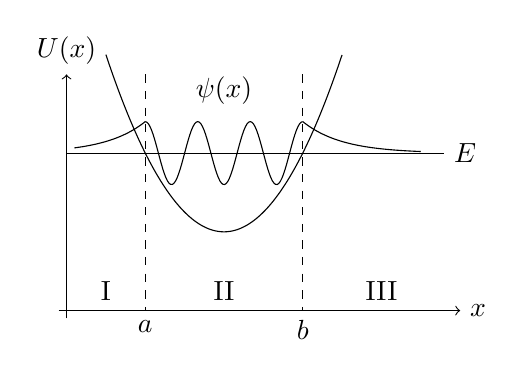
\begin{tikzpicture}[domain=0:5]
    \draw[->] (-0.1,0) -- (5,0) node[right] {$x$};
    \draw[->] (0,-0.1) -- (0,3) node[above] {$U(x)$};
	\draw [domain=0:4.8, samples=50] plot (\x, {2}) node[right] {$E$};
	\draw [domain=0.5:3.5, samples=100] plot (\x, {(\x-1)*(\x-3)+2});
  \draw [domain=1.0:3.0, samples=100] plot (\x, {0.4*sin(540*\x+270)+2});
	\draw [domain=0.1:1.0, samples=100] plot (\x, {0.4*exp(2*\x-2)+2});
	\draw [domain=3.0:4.5, samples=100] plot (\x, {0.4*exp(-2*\x+6)+2});
  \draw[dashed] (1,3) -- (1,0) node[below] {$a$};
  \draw[dashed] (3,3) -- (3,0) node[below] {$b$};
	\draw (2,2.5) node[above] {$\psi(x)$};
	\draw (0.5,0) node[above] {I};
	\draw (2,0) node[above] {II};
  \draw (4.0,0) node[above] {III};
\end{tikzpicture}
\caption{К выводу условий квантования Бора-Зоммерфельда} \label{fig:11_4}
\end{figure}

\underline{Физическое условие}: на $\pm \infty$ решения должны убывать. Поэтому при переходе во внутреннюю область (область ямы) применим при $x=a$, $x=b$ правило соответствия \rom{1}:

$$
\begin{gathered}
\Psi_{x<b}(x) = \frac{a_1}{\sqrt{p}} \sin\brs{\frac{1}{\hbar} \int_{x}^{b} p(x')dx' + \frac{\pi}{4} } \equiv \frac{a_1}{\sqrt{p}} \sin({z_1 + \frac{\pi}{4}}) \\
\Psi_{x>a}(x) = \frac{a_2}{\sqrt{p}} \sin\brs{\frac{1}{\hbar} \int_{a}^{x} p(x')dx' + \frac{\pi}{4} } \equiv \frac{a_2}{\sqrt{p}} \sin({z_2 + \frac{\pi}{4}})
\end{gathered}
$$

где $z_1+z_2 = \dfrac{1}{\hbar} \int \limits_{a}^{b} p(x')dx' \equiv \dfrac{1}{\hbar} \int \limits_{a}^{b} p(x)dx$.

Этим решения должны совпадать во всей области $a < x < b$.
$$
\begin{aligned}
\frac{a_1}{\sqrt{p}} \sin({z_1+\frac{\pi}{4}}) = \frac{a_2}{\sqrt{p}} \sin({z_2+\frac{\pi}{4}}) = \frac{a_2}{\sqrt{p}} \sin\brs{\frac{1}{\hbar} \int_{a}^{b} p(x)dx - z_1 + \frac{\pi}{4}} = \\
= -\frac{a_2}{\sqrt{p}} \sin\brs{z_1 - \frac{1}{\hbar} \int_{a}^{b} p(x)dx - \frac{\pi}{4} }
\end{aligned}
$$

\begin{equation}
\label{eq:11_3_1}
z_1 + \frac{\pi}{4} = z_1 - \frac{1}{\hbar} \int_{a}^{b} p(x)dx - \frac{\pi}{4} + \pi(n+1) ~~ n \in \cal{N} \\
\end{equation}
\begin{equation}
\label{eq:11_3_2}
a_1 = (-1)(-1)^{n+1}a_2  ~~\rightarrow~~ a_2 = a_1 (-1)^n
\end{equation}

В условии \eqref{eq:11_3_1} пишем $\pi (n+1)$, а не $\pi n$ т.к. при $n=0$ было бы $\dfrac{1}{\hbar}\int \limits_{a}^{b} p(x) dx = -\dfrac{\pi}{2}$, что не допустимо, так как левая часть этого равенства - заведомо положительная величина.

Таким образом, 
\begin{equation}
\label{eq:11_3_3}
\boxed{\int_{a}^{b} p(x)dx = \pi\hbar\brc{n+\frac{1}{2}}}
\end{equation}

или взятый по полному периоду классического движения частицы между точками $x=a$ и $x=b$ интеграл $\oint p(x)dx \equiv 2 \int \limits_{a}^{b} p(x)dx$ равен
\begin{equation}
\label{eq:11_3_4}
\boxed{\oint p(x)dx = 2\pi\hbar\brc{n+\frac{1}{2}}}
\end{equation}

Соотношения \eqref{eq:11_3_3}, \eqref{eq:11_3_4} есть правило квантования Бора-Зоммерфельда из старой квантовой теории, предложенной в 1915 году еще до создания квантовой механики. Т.к. $p(x) = \sqrt{2m(E_n - U(x))}$, то это правило определяет энергии $E_n$ стационарных состояний квантовой системы в квазиклассическом приближении.

\begin{enumerate}
\item Правило \eqref{eq:11_3_4} есть квантование адиабатических инвариантов. В квантовой механике при медленном (адиабатическом) изменении параметров системы она остается в том же квантовом состоянии ($n = const$). Это согласуется с теоремой в классической механике о постоянстве адиабатических инвариантов при медленном изменении параметров системы (\llref{49}{1}).

\item Номер состояния $n$: $n \to E_n$. Но это целое число не только порядковый номер стационарного состояния, но и число нулей (узлов) волновой функции. Действительно, при продвижении по $x$ от $a$ к $b$ фаза волновой функции растет от $\dfrac{\pi}{4}$ до $\dfrac{1}{\hbar} \left. \int \limits_{a}^{b} p(x)dx + \dfrac{\pi}{4} \right|_{\text{\eqref{eq:11_3_3}}} =\pi n + \dfrac{3}{4}\pi$, так что синус обращается на этом интервале в нуль $n$ раз (вне интервала $a < x < b$ волновая функция монотонно затухает (\autoref{fig:11_4}), не имея нулей). Это есть частный случай осцилляционной теоремы квантовой механики(глава \rom{7}, \textsection{3}).
\end{enumerate}

Но пользоваться квазиклассическим приближением можно лишь тогда, когда между точками поворота укладывается достаточно много длин волн $\lambdabar = \dfrac{\hbar}{p(x)}$ (хотя бы потому, что от каждой из точек поворота нужно отступить на расстояния порядка нескольких длин волн, когда справедливы асимптотические решения типа $\sin \brs{z + \dfrac{\pi}{4}}$). Поскольку расстояние между узлами волновой функции $\sim \lambdabar$, а выше в методе ВКБ использовался безразмерный малый параметр $\dfrac{\lambdabar}{L} \ll 1$ (здесь $L$-характерный размер квантовой системы), то в квазиклассическом приближении $\dfrac{\lambdabar}{L} \sim \boxed{n \gg 1}$.

В связи с изложенным выше возникает вопрос, а законно ли в таком приближении рядом с $n$ удерживать $\dfrac{1}{2}$ в формулах \eqref{eq:11_3_3}, \eqref{eq:11_3_4}? Поскольку все полученные ранее результаты справедливы в линейном по $\hbar$ приближении (см. \textsection{2.1} этой главы), когда $\dfrac{\lambdabar}{L} \sim \dfrac{1}{n} \ll 1 \sim \dfrac{1}{2}$, то поправка к числу узлов $\dfrac{1}{2}$ на самом деле имеет точность $\sim \dfrac{1}{n}$, так что удерживать ее на фоне такой точности при $n \gg 1$ в правой части формул \eqref{eq:11_3_3}, \eqref{eq:11_3_4} законно.

\section{Фазовый объём, приходящийся на одно квантовое состояние}

Соотношение \eqref{eq:11_3_4} можно истолковать и другим образом. $\oint p(x)dx$ есть площадь в фазовом пространстве $(p,x)$ частица, охватывающая квантовые состояния, энергия которых $E \le E_n$. При переходе $E_n \to E_{n+1}$ область фазового пространства увеличивается на $2\pi\hbar$. Значит, на одно квантовое состояние в фазовом пространстве приходится <<клетка>> площадью $2\pi \hbar$:
$$
\boxed{\Delta\Gamma = 2\pi\hbar}
$$

Иными словами, число квантовых состояний, отнесенное к элементу фазового объема $\Delta p \Delta x$.
$$
\boxed{\Delta N = \frac{\Delta p \Delta x}{2\pi\hbar}}
$$

\begin{sloppypar}
  \section{Вероятность проникновения частицы через барьер в квазиклассическом приближении}
\end{sloppypar}

Пусть имеется гладкий потенциальный барьер, т.е. между классически разрешенными областями \rom{1} и \rom{3} находится классически запрещенная область \rom{2}, где $E < U(x)$. В квантовой механике в силу волновых свойств частиц барьер обладает прозрачностью. Пусть выполнены условия квазиклассичности, т.е. барьер очень широк, и, как следствие, коэффициенто прохождения мал. 

\begin{figure}[h]
\centering
\includegraphics[scale=1]{figs/11_5}
\caption{Проникновение частицы через барьер}
\label{fig:11_5}
\end{figure}

\begin{enumerate}
\item В области \rom{3} есть квазиклассическая волна, бегущая слева направо:
$$
\Psi_{x>b}(x) \simeq \frac{A}{\sqrt{p(x)}} \exp\brc{\frac{i}{\hbar} \int_{b}^{x} p(x')dx' + i\frac{\pi}{4}}
$$

Убедимся в том, то это действительно так. В соответствии с \textsection{1} главы \rom{5} плотность потока вероятности прошедшей волны
$$
\begin{aligned}
j_{x}^{\text{прош}} = \frac{i\hbar}{2m}(\psi\nabla\psi^* - \psi^*\nabla\psi) = \brc{\text{т.к. слагаемые}~ \sim \nabla \frac{1}{\sqrt{p(x)}} ~\text{взаимно компенсируются}} =\\
= \frac{i\hbar}{2m} \brcr{\frac{A}{\sqrt{p(x)}} e^{i\brs{z(x)+\frac{\pi}{4}}} \frac{A^*}{\sqrt{p(x)}} e^{-i\brs{z(x)+\frac{\pi}{4}}} \brc{-i\frac{dz}{dx}} - \brc{\text{комплексно-сопряженное}} } = \\
= \frac{i\hbar}{2m} \brcr{\frac{-i\abs{A}^2 2}{\hbar}} = \frac{\abs{A}^2}{m} = j_x^{\text{прош}} > 0
\end{aligned}
$$

\item В области \rom{2} по правилу соответствия (\rom{3}):
$$
\Psi_{a<x<b}(x) \simeq \frac{A}{\sqrt{\abs{p}}} \exp\brc{\frac{1}{\hbar} \int_x^{b} \abs{p(x')}dx'} \equiv 
$$
$$
\equiv \frac{A}{\sqrt{\abs{p}}} \underbrace{ \exp\brc{\frac{1}{\hbar} \int_{a}^{b} \abs{p(x')}dx'} }_{e^{\gamma}} \exp\brc{- \frac{1}{\hbar} \int_{a}^{x} \abs{p(x')}dx'}
$$

\item В области \rom{1} по правилу соответствия (\rom{1}):
$$
\Psi_{x<a}(x) \simeq \frac{2A}{\sqrt{p}} \sin\brs{\frac{1}{\hbar} \int_{x}^{a} p(x')dx' + \frac{\pi}{4}} e^{\gamma} =
$$
$$
= \frac{2A e^{\gamma}}{\sqrt{p}} \left\{ \underbrace{\exp \brc{\frac{i}{\hbar} \int_{x}^{a} p(x')dx' + \frac{i\pi}{4}}}_{\text{отраженная волна}} - \underbrace{\exp \brc{-\frac{i}{\hbar} \int_{x}^{a} p(x')dx' - \frac{i\pi}{4}}}_{\text{падающая волна}}\right \} 
$$
$$
j_x^{\text{пад}} = \frac{i \hbar}{2m} \brcr{\Psi \nabla \Psi^* - \Psi^* \nabla \Psi} = \frac{i \hbar}{2m} \brcr{\frac{A e^{\gamma}}{i \sqrt{p}} e^{-i(z(x) + \frac{\pi}{4})} \frac{A^* e^{\gamma}}{(-i) \sqrt{p}} e^{i(z(x) + \frac{\pi}{4})} \brc{i \frac{dz}{dx}} - \text{К.С.} } =
$$
$$
= \frac{i \hbar}{2m} \brcr{\frac{-2i \abs{A}^2 e^{2\gamma}}{\hbar}} = \frac{\abs{A}^2 e^{2\gamma}}{m}
$$

\item По определению коэффициент проницаемости барьеры (или вероятность проникновения частицы через барьер):
$$
\boxed{D \equiv \frac{\abs{j_x^{\text{прош}}}} {\abs{j_x^{\text{пад}}}} = e^{2\gamma} = e^{-\frac{2}{\hbar} \int_a^b \abs{p(x)} dx}} 
$$
- формула впервые в 1928 году была получена Георгием Антоновичем Гамовым в связи с теорией радиоактивного $\alpha$-распада ядер.

Коэффициент отражения в таком подходе:
$$
R \equiv \frac{\abs{j_x^{\text{отр}}}}{\abs{j_x^{\text{пад}}}} = 1
$$
- амплитуды падающей и отраженной волн в области \rom{1} оказались одинаковыми. Его фактическое отличие от 1 не может быть найдено в рамках квазиклассического приближения, т.к. здесь всегда теряются экспоненциально убывающие решения на фоне экспоненциально растущих в области \rom{2}. В этой связи формула Гамова применима, если показатель экспоненты велик, $2\gamma \gg 1$, так что сам $D \ll 1$.
\end{enumerate}
